\subsubsection{Continental extension}
\label{sec:cookbooks-continental-extension}
\textit{This section was contributed by John Naliboff}

In the crustal deformation examples above, the viscosity depends solely on the Drucker Prager yield criterion defined by the cohesion and internal friction angle. While this approximation works reasonably well for the uppermost crust, deeper portions of the lithosphere may undergo either brittle or viscous deformation, with the latter depending on a combination of composition, temperature, pressure and strain-rate. In effect, a combination of the Drucker-Prager and Diffusion dislocation material models is required. The visco-plastic material model is designed to take into account both brittle (plastic) and non-linear viscous deformation, thus providing a template for modeling complex lithospheric processes. Such a material model can be used in \aspect{} using the following set of input parameters:

\lstinputlisting[language=prmfile]{cookbooks/continental_extension/doc/continental_extension_material_model.prm.out}

This cookbook provides one such example where the continental lithosphere undergoes extension. Notably, the model design follows that of numerous previously published continental extension studies~\cite[and references therein]{Hui11,Bru14,Nal15}.

\paragraph{Continental Extension}
The 2D Cartesian model spans 400 (x) by 100 (y) km and has a finite element grid with uniform 2 km spacing. Unlike the crustal deformation cookbook (see Section~\ref{sec:cookbooks-crustal-deformation}, the mesh is not refined with time.

\lstinputlisting[language=prmfile]{cookbooks/continental_extension/doc/continental_extension_geometry_mesh.prm.out}


Similar to the crustal deformation examples above, this model contains a free surface. Deformation is driven by constant horizontal ($x$-component) velocities (0.25 cm/yr) on the side boundaries ($y$-velocity component unconstrained), while the bottom boundary has vertical inflow to balance the lateral outflow. The top, and bottom boundaries have fixed temperatures, while the sides are insulating. The bottom boundary is also assigned a fixed composition, while the top and sides are unconstrained.

\lstinputlisting[language=prmfile]{cookbooks/continental_extension/doc/continental_extension_boundary_conditions.prm.out}

Sections of the lithosphere with distinct properties are represented by compositional fields for the upper crust (20 km thick), lower crust (10 km thick) and mantle lithosphere (70 km thick). A mechanically weak seed within the mantle lithosphere helps localize deformation. Material (viscous flow law parameters, cohesion, internal friction angle) and thermodynamic properties for each compositional field are based largely on previous numerical studies.   Dislocation creep viscous flow parameters are taken from published deformation experiments for wet quartzite \cite{RB04}, wet anorthite \cite{RGWD06} and dry olivine \cite{HK04}.

\lstinputlisting[language=prmfile]{cookbooks/continental_extension/doc/continental_extension_composition.prm.out}

The initial thermal structure, radiogenic heating model and associated thermal properties are consistent with the prescribed thermal boundary conditions and produce a geotherm characteristic of the continental lithosphere. The equations defining the initial geotherm \cite{Cha86} follow the form
\begin{align}
  \label{eq:continental-geotherm-1}
  T(z) &= T_T + \frac{q_T}{k}z - \frac{Az^2}{2k}
\end{align}
where $T$ is temperature, $z$ is depth, $T_T$ is the temperature at the layer surface (top), $q_T$ is surface heat flux, $k$ is thermal conductivity, and $A$ is radiogenic heat production.

For a layer thickness $\Delta z$, the basal temperature ($T_B$) and heat flux ($q_B$) are
\begin{align}
  \label{eq:continental-geotherm-2}
  T_B &= T_T + \frac{q_T}{k} \Delta z - \frac{A \Delta z^2}{2k},
  \\
  \label{eq:continental-geotherm-3}
  q_B &= q_T - A \Delta z.
\end{align}

In this example, specifying the top (\SI{273}{K}) and bottom temperature (\SI{1573}{K}), thermal conductivity of each layer and radiogenic heat production in each layer provides enough constraints to successively solve for the temperature and heat flux at the top of the lower crust and mantle.

As noted above, the mechanically weak seed placed within the mantle localizes the majority of deformation onto two conjugate shear bands that propagate from the surface of the seed to the free surface. After 5 million years of extension background `stretching' is clearly visible in the strain-rate field, but deformation is still largely focused within the set of conjugate shear bands originating at the weak seed  (Fig.~\ref{fig:continental_extension_cookbook_strainrate_5e6yr}). As expected, crustal thickness and surface topography patterns reveal a relatively symmetric horst and graben structure, which arises from displacements along the shear bands (Fig.~\ref{fig:continental_extension_cookbook_composition_5e6yr}). While deformation along the two major shear bands dominates at this early stage of extension, additional shear bands often develop within the horst-graben system leading to small inter-graben topographic variations. This pattern is illustrated in a model with double the numerical resolution (initial 1 km grid spacing) after 10 million years of extension  (Fig.~\ref{fig:continental_extension_cookbook_strainrate_highres_10e6yr}).

With further extension for millions of years, significant crustal thinning and surface topography development should occur in response to displacement along the conjugate shear bands. However, given that the model only extends to 100 km depth, the simulation will not produce a realistic representation of continental breakup due to the lack of an upwelling asthenosphere layer. Indeed, numerical studies that examine continental breakup, rather than just the initial stages of continental extension, include an asthenospheric layer or modified basal boundary conditions (e.g. Winkler boundary condition \cite[for example]{Bru14})
as temperature variations associated with lithospheric thinning exert a first-order influence on the deformation patterns. As noted below, numerous additional parameters may also affect the temporal evolution of deformation patterns.

\note{It is important to consider that the non-linearity of visco-plastic rheologies and mesh-dependence of brittle shear bands make lithospheric deformation models highly sensitive to a large number of parameters. In order to ensure the conclusions drawn from a series of numerical experiments are robust, one should complete a sensitivity test for a large range of parameters including grid resolution, model geometry, boundary conditions, initial composition and temperature conditions, material properties, composition discretization, CFL number and solver settings. If you are new to modeling lithospheric processes, a reasonable starting point is to try and reproduce results from a relevant previous study and then perform a sensitivity test for the parameters listed above. While highly time consuming, completing this procedure will prove invaluable when you design and assess the results of your own numerical study.}

\begin{figure}
\centering
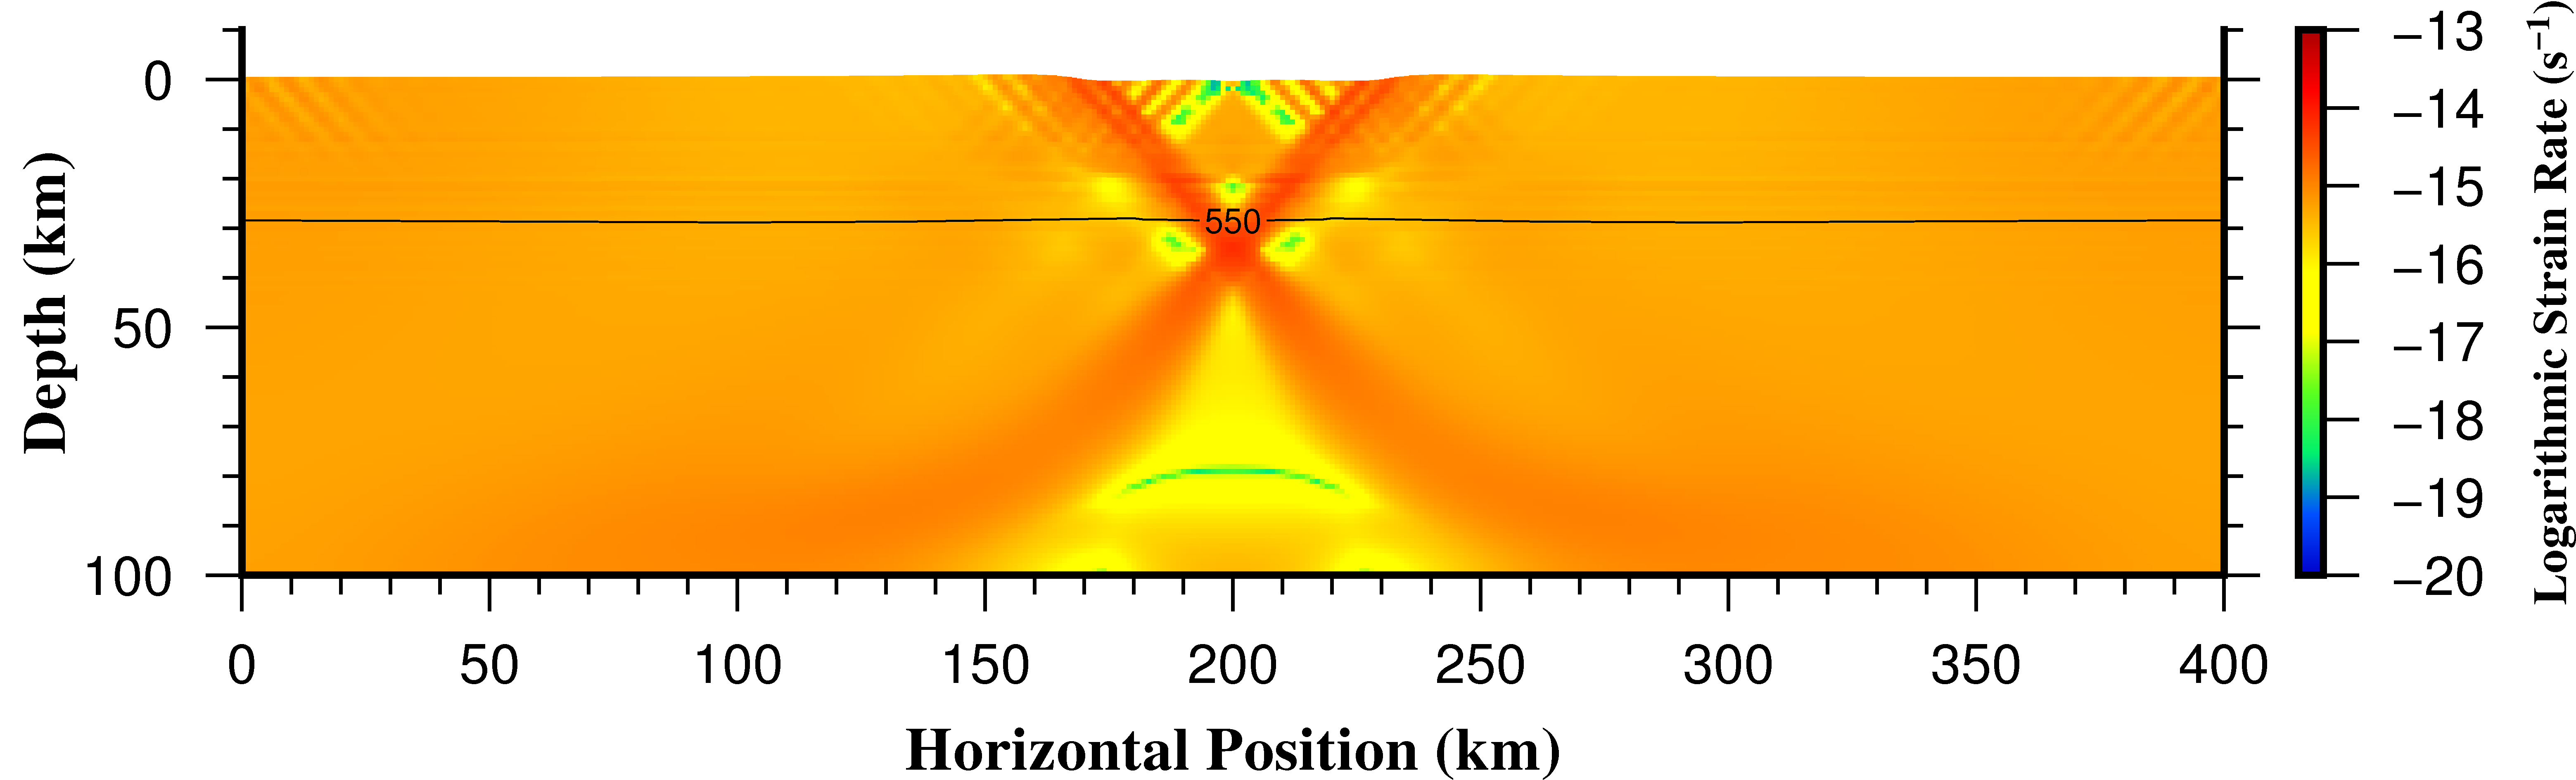
\includegraphics[width=\textwidth]{cookbooks/continental_extension/doc/continental_extension_cookbook_strainrate_5e6yr.png}
\caption{\it Strain rate (in units of $s^{-1}$) after \num{5e6} years of extension. The black line marks the 550 $\degree C$ isotherm.}
\label{fig:continental_extension_cookbook_strainrate_5e6yr}
\end{figure}
\begin{figure}
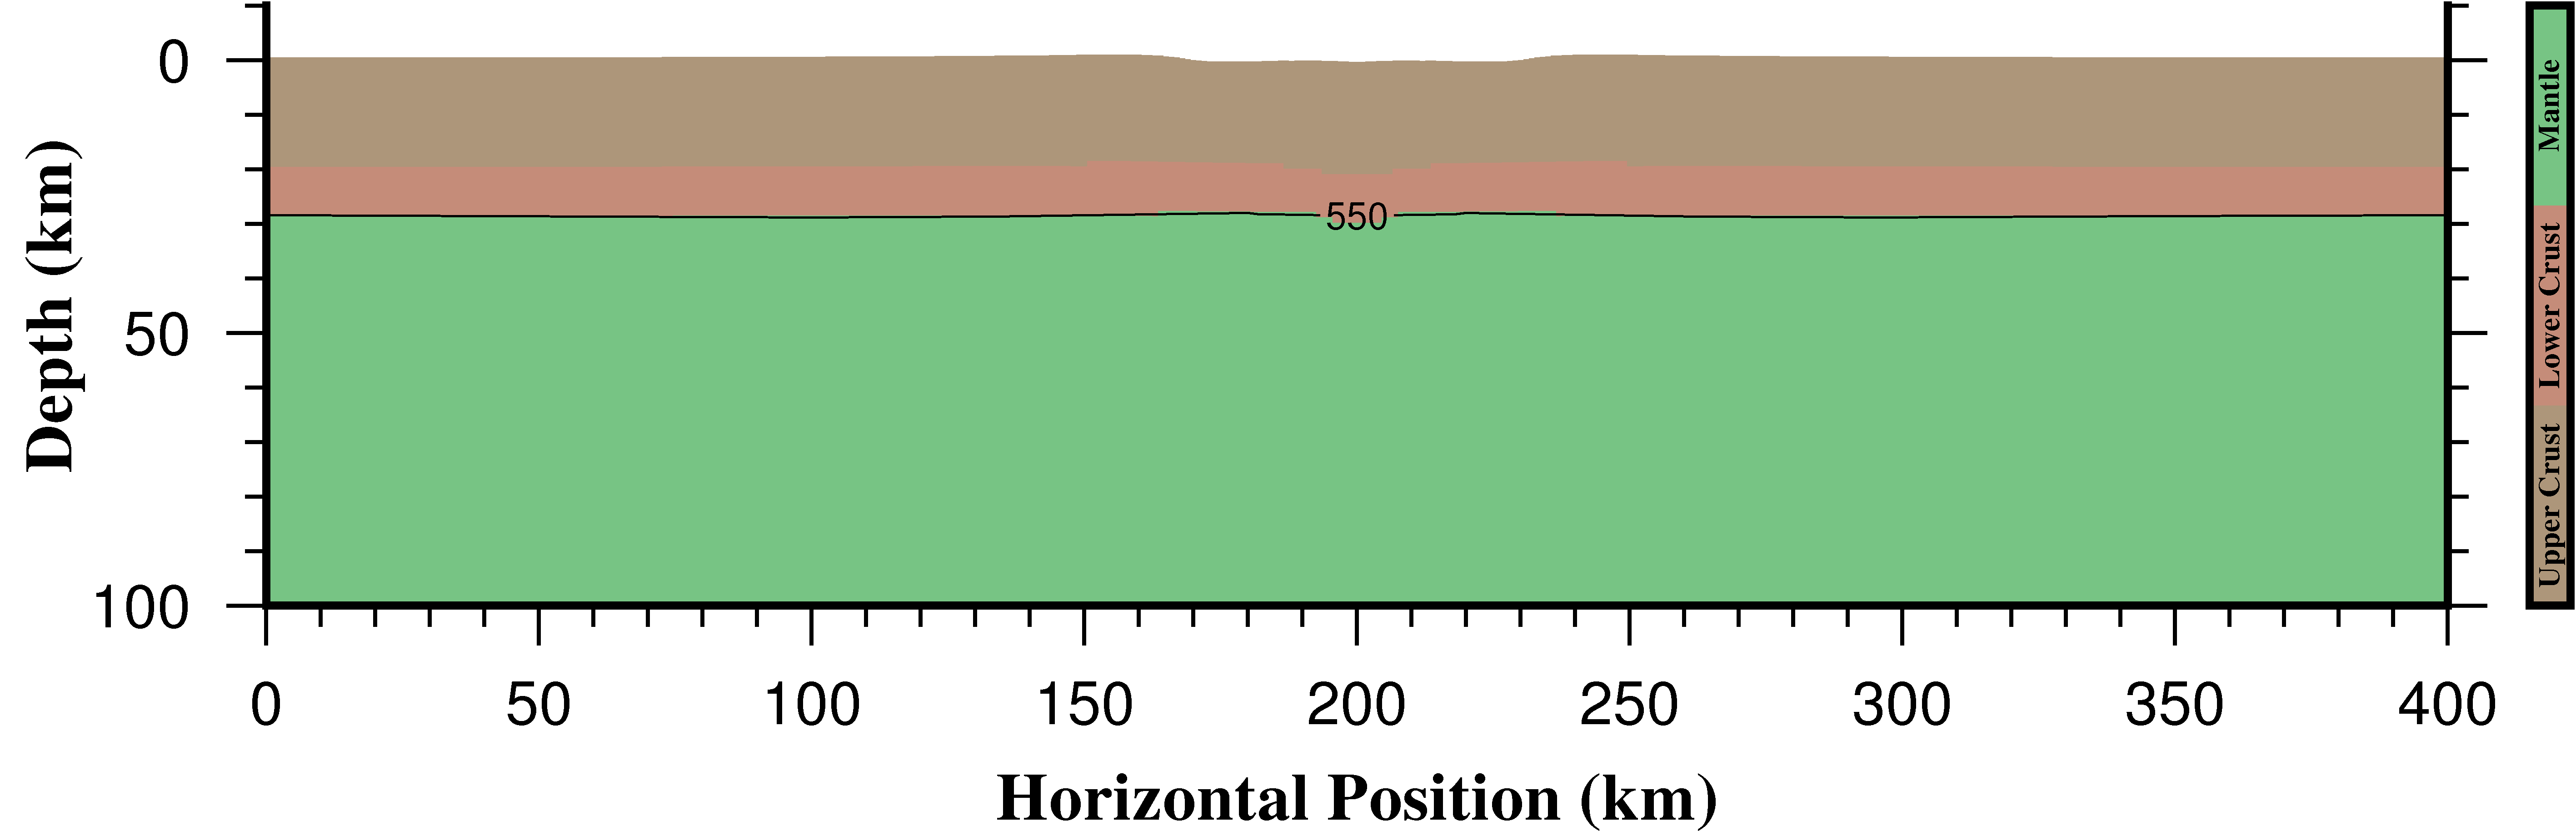
\includegraphics[width=\textwidth]{cookbooks/continental_extension/doc/continental_extension_cookbook_composition_5e6yr.png}
\caption{\it Compositional field after \num{5e6} years of extension. The black line marks the 550 $\degree C$ isotherm.}
\label{fig:continental_extension_cookbook_composition_5e6yr}
\end{figure}
\begin{figure}
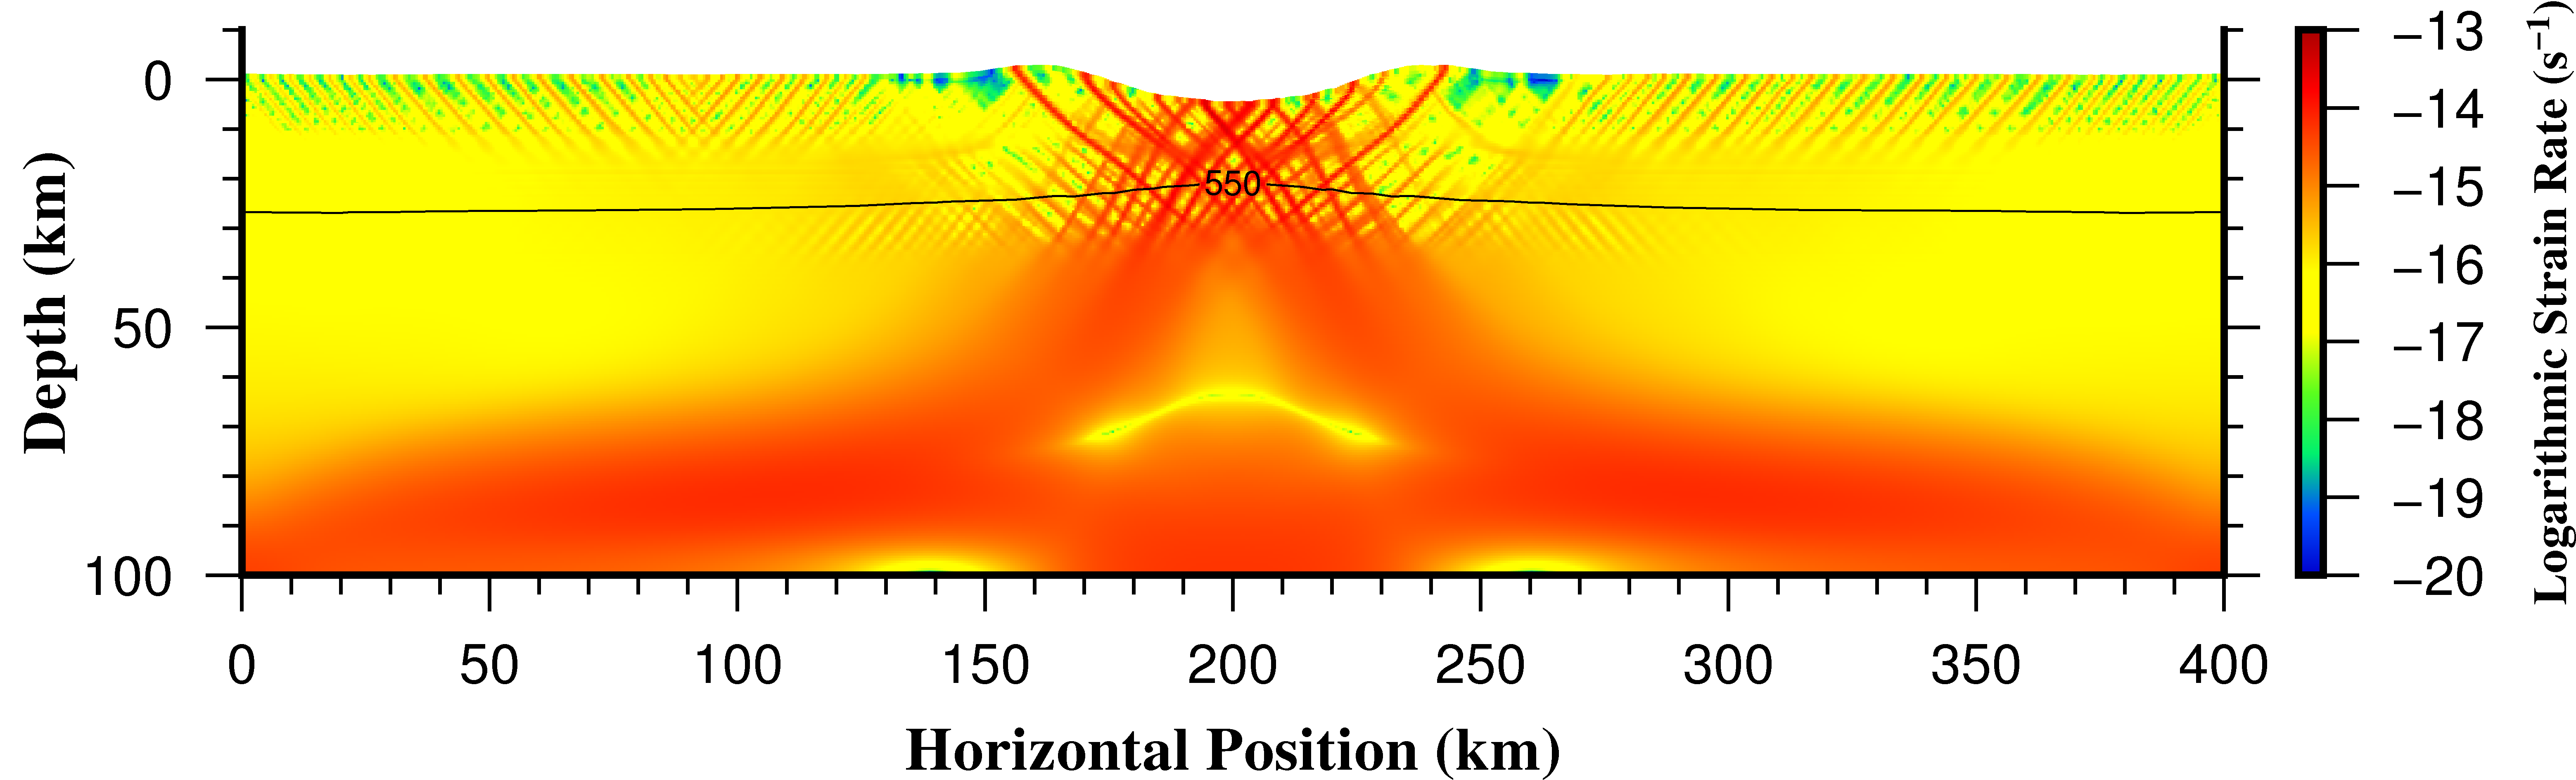
\includegraphics[width=\textwidth]{cookbooks/continental_extension/doc/continental_extension_cookbook_strainrate_highres_10e6yr.png}
\caption{\it Strain rate (in units of $s^{-1}$) after \num{10e6} years of extension. The black line marks the 550 $\degree C$ isotherm. The numerical resolution ($1 \si{km}$) is double that of the previous model.}
\label{fig:continental_extension_cookbook_strainrate_highres_10e6yr}
\end{figure}

